\section{Data Acquisition}
\label{section:data}

The data acquisition component of \textit{GESTALT} begins with a visual and geospatial encoding of the world. 
%The visual encoding is primarily remote sensing imagery providing a top-down view of the earth's surface, but it also includes street-view imagery and other photographs. 

\emph{GESTALT} enables last-mile search within a given \emph{region}, using two types of geotags: \emph{object} tags and \emph{location} tags.

\emph{Regions} represent a limited physical area of interest within which last-mile search is to be performed. ........anything else to the definition? scope? size?..................


\emph{Objects} represent any physical entity located within the region of interest. For example, a \textit{tree, building, lake, bridge, gate} or \textit{sign} could be an object. \textit{Objects} can also have attributes that provide amplifying information about them, including things like \textit{color, material, size, species etc.}. 

\emph{Locations} represent physical entities that \textit{do} something. They are a meaningful grouping of objects determined by ownership, proximity or utility. They have some purpose beyond that of objects. Examples of locations include \textit{businesses, attractions, properties etc.}. \textit{Locations} own \textit{objects}, and \emph{GESTALT} enables users to query for locations given a partial set of knowledge about the objects at those locations.

\subsection{Object Tags}
To maximize dataset coverage, and demonstrate the flexibility of \emph{GESTALT} we support three methods of ingesting objects:
\begin{enumerate}
    \item Ingesting KML Files that contain manually annotated objects and their coordinates 
    \item Querying the Open Street Maps (OSM) API to ingest crowd-sourced object tags and their coordinates
    \item Automatically detecting objects in geolocated photos pulled from the Flickr API 
\end{enumerate}

Upon ingest, each object is assigned a confidence score, reflecting the certainty that the object tagged at those coordinates actually exists and is of the type annotated. 
For results reported in this paper, we adopt the rule that hand-labeled objects receive a confidence score of $1.0$, OSM objects receive a score of $0.75$ and objects labeled by the object detector receive the confidence score reported by the object detection model. Table~\ref{table:objects} contains a summary of the objects currently in \emph{GESTALT}.


\begin{table}[h!]
	\begin{center}
		\begin{tabular}{ |c|c|c|c| } 
			\hline
			 Source & Ingest Method & Quantity & Num distinct classes  \\
			\hline
                Swan Valley Wineries & Hand-labeled & $?????$ & $?????$ \\ 
			.................... & Hand-labeled & $?????$ & $?????$  \\ 
                .................... & OSM Query & $?????$ & $?????$ \\ 
			Flickr ........ & Object detection & $?????$ & $?????$  \\ 
			\hline
		\end{tabular}	
		\caption{..............}
            \label{table:objects}
	\end{center}
\end{table} 

\subsection{Location Tags}
We support two methods of ingesting locations:
\begin{enumerate}
    \item Ingesting KML Files that contain manually annotated locations and their coordinates 
    \item Querying the Open Street Maps (OSM) API to ingest crowd-sourced location tags and their coordinates 
\end{enumerate}

.................. confidence scores?..................and do we use hand-labeled locs or do they come from OSM also? ...............................

\subsection{Ingest Methods}
\subsubsection{Ground Truth Hand Labeled Tags} 
Hand labeled objects and locations are those that have been manually annotated by a trustworthy source, and are assumed to be correctly labeled and correctly geotagged. 
The reason we accept hand-labeled tags is to allow for prior manual annotation work to be folded into \emph{GESTALT}'s database, and to provide a reliable means to report results on ground truth data, so that we can compare \emph{GESTALT} with future architectures that might attempt to solve the last-mile search problem with a different approach. 

For benchmarking purposes we curated the \emph{Swan Valley Wineries} dataset containing ground truth object tags, location tags, and the correct associated between them (i.e. which objects belong to which locations) for six wineries within the Swan Valley Region of Western Australia.
%NSCH need better transitions in the below chunk about wineries tags
The wineries tags are stored in Keyhole Markup Language~\footnote{\href{https://developers.google.com/kml/documentation/kml\_tut}{https://developers.google.com/kml/documentation/kml\_tut}} (KML).
The tags consist of an object name, its latitude \& longitude, and any descriptive markings written as key:value pairs. The objects are stored by their ground truth parent location in a KML file.
The object tagging was conducted manually by a single annotator, combining on-the-ground knowledge with manual inspection of satellite imagery, street-view imagery and publicly available photos of the area. 
The objects tagged are representative, not exhaustive. 
The object tags are aligned with ..................................... 
The tagging was conducted using \textit{Google Earth Professional version 7.3\footnote{\href{https://www.google.com/earth/about/versions/}{https://www.google.com/earth/about/versions/}}}
Attributes of the objects (e.g. color, size, material) are recorded in the comments field as key:value pairs.
Each object from the hand-labeled dataset is assigned a confidence score of 1.0, since it was manually identified and tagged.

%NSCH: is the below sentence about the labeling or the module that aggregates all the sources? Or no longer relevant?
%The KML parser leverages the \textit{fastKML}\footnote{\href{https://pypi.org/project/fastkml/}{Fast KML PyPI Repo}} and ingests a KML file divided by region (where each region is a bounding box covering an arbitrary number of locations). 


% NSCH need to place and introduce/discuss these plots
\begin{figure*}[ht]
    \label{fig:loc}        
    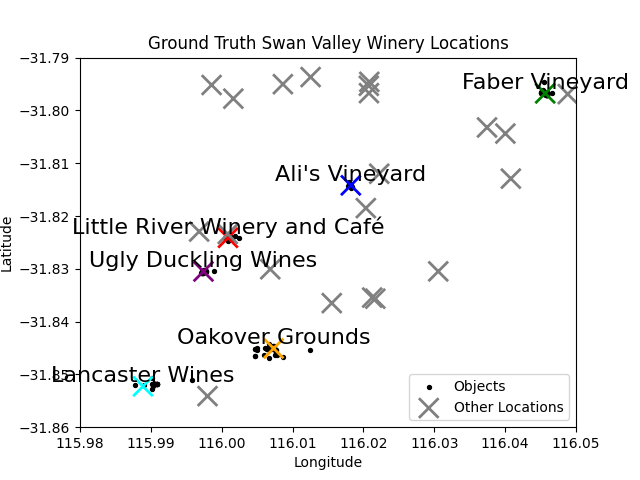
\includegraphics[width=0.5\textwidth]{loc_labels_plot.png}
    \centering
    \caption[width=\textwidth]{............}
\end{figure*}


\begin{figure*}[ht]
    \label{fig:loc-obj}        
    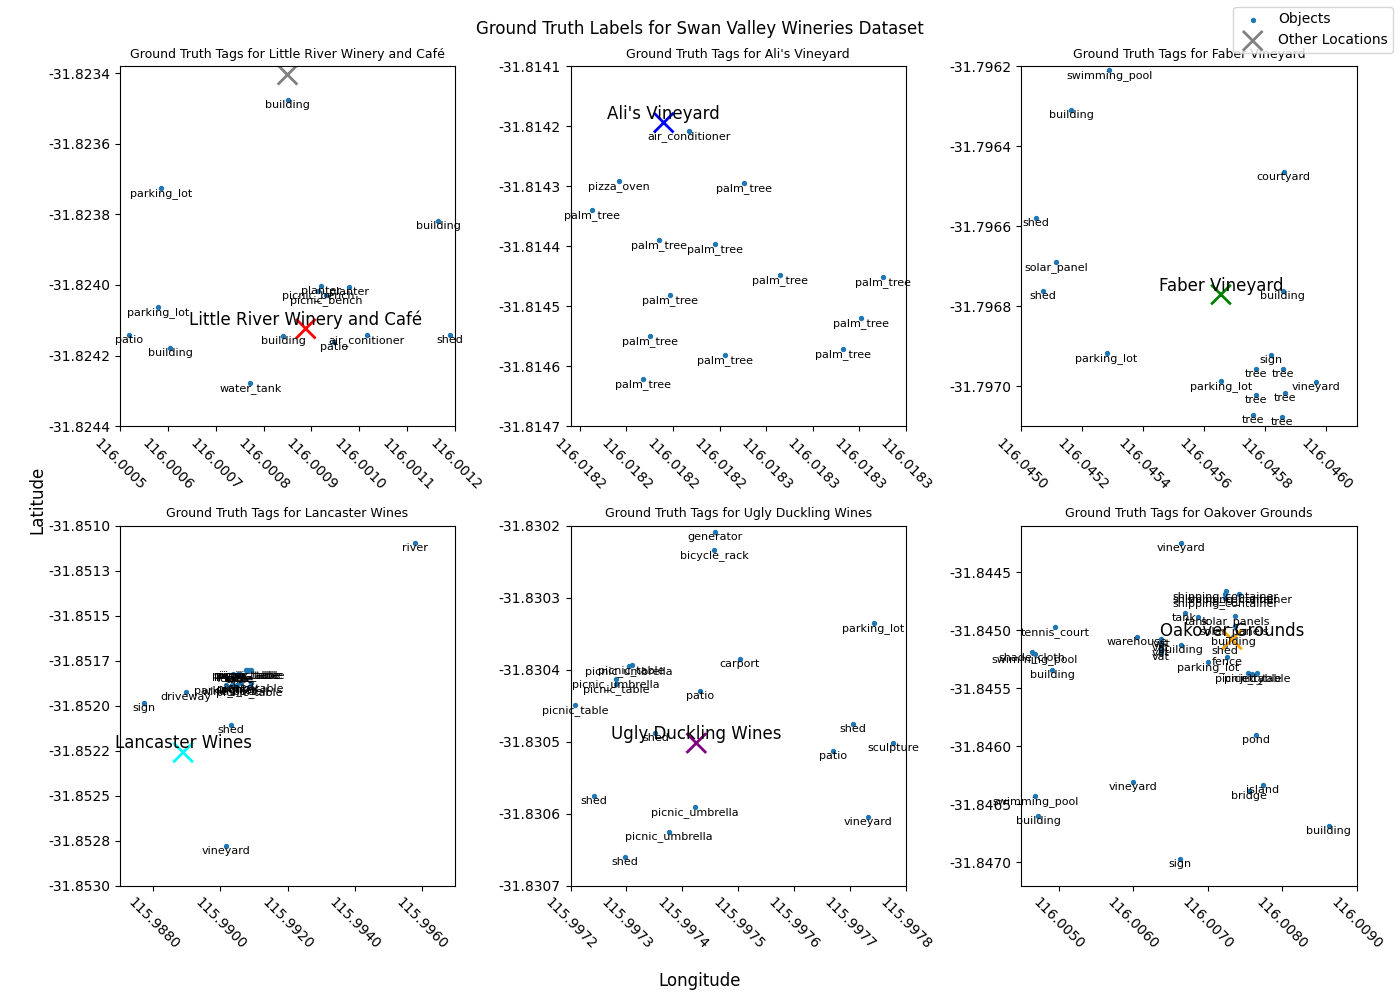
\includegraphics[width=\textwidth]{loc_obj_labels_plot.png}
    \centering
    \caption[width=\textwidth]{............}
\end{figure*}


\subsubsection{Open Street Maps Tags}
\emph{GESTALT} can ingest object and location tags by querying the Open Street Maps (OSM) API.
OSM is a knowledge collective that contains open-source Geodata~\cite{Haklay2008}, which can be easily extended via their online editing interface.
While businesses, attractions and other \textit{locations} are commonly annotated by the OSM community, \textit{objects} are more sparsely tagged, since few people have the patience to manually label apparently inconsequential things like trees, statues, fountains and telephone poles. 
\emph{GESTALT} ingests what object tags do exist in OSM through 
............describe the process here (API? fields queried? post-processing?)....................
Each object ingested from OSM is assigned a confidence score of 0.75, since these tags are maintained by the open-source community and are subject to a combination of human review and an application of machine learning for detecting anomalous behavior in OSM edits~\cite{Mooney2017}, but can still be wrong in many cases~\cite{VargasMunoz2020}.
Describe how locations are ingested...................fields used?..............%The OSM query interface leverages the \textit{OSMPythonTools}\footnote{\href{https://pypi.org/project/OSMPythonTools/}{OSMPythonTools PyPI Repo}}. It passes a bounding box to the OSM Overpass-Turbo API\footnote{\href{https://overpass-turbo.eu/}{Overpass-Turbo API}} and requests the relevant location nodes in the area.
Businesses, attractions and other higher-level \textit{locations} are commonly annotated in OSM by the open-source community or business owners themselves.
%NSCH need to cut/clean up the below chunk about OSM
OSM records objects' coordinates as a mixture of point coordinates and bounding polygons. 
OSM has a defined and curated ontology that defines the labeling scheme, maximizing interoperability. 
The OSM objects are crowd-sourced and of varying granularity and completeness. Incompleteness is part of the initial scope of OSM, with the founder noting that it's typically only what people want to add that gets added \cite{Haklay2008}.
In general, the completeness of OSM is unassured, so scaling \textit{GESTALT} beyond the trivial requires an automated method for object detection and resolution. 


\subsubsection{Noisy Image-based Tags}
The third, and most important method by which \emph{GESTALT} ingests objects, is through automatic object detection.
Given a set of images and their associated geo data, ...........what is it actually called?........... the Object Detection module uses YOLO~\footnote{\href{https://github.com/ultralytics/ultralytics}{YOLO}} to identify objects in each image. Those objects are then tagged with the geolocation of the image, and stored...........how?........... For our experiments, we pull ..............how many?............ images over ............timeframe.......... and use pre-trained YOLO v.8 to detect objects from 80 classes (based on the COCO dataset.........footnote........). Each object identified is assigned a probability score ...........how does YOLO get that????..........



%An automated solution aims to leverage publicly available remote sensing imagery data (Bing Maps Satellite data, for example) and public streetview and photo contributions to automatically identify objects, geo-locate them and add those tags to a database. 
%The design for this subsystem breaks maps into small geographically-bounded chunks (approximately the size of a 'location'). 
%It will use remote-sensing imagery to create a grid of objects / not-object. It will retrieve ground-level imagery within and adjacent to that box.


%The data extraction, cleaning and loading are implemented in Python in two parts, the \textit{KML parser} for object extraction and the \textit{Open Street Maps} query interface for location retrieval. 
%The KML parser leverages the \textit{fastKML}\footnote{\href{https://pypi.org/project/fastkml/}{Fast KML PyPI Repo}} and ingests a KML file divided by region (where each region is a bounding box covering an arbitrary number of locations). 
%Within each region (for this test dataset), each location is separated, with its objects stored as its children. 
%Attributes of the objects (e.g. color, size, material) are recorded in the comments field as key:value pairs.
%The KML Parser extracts the objects into dictionaries organized by location before exporting the files as JSON for future analysis. 

%Google Maps\footnote{\href{https://www.google.com/maps/about/}{Google Maps}} maintains \textit{locations} as coordinate points with associated metadata. The locations are generally current and complete. 
%Google Maps does not support bounding polygons at the location level; it appears to extend to as granular as ZIP Codes or suburb boundaries and no further. 
%OSM Supports locations, but is less complete than Google Maps (at least for Australian Wine Regions.)
%In general, for \textit{GESTALT} to function optimally, the input locations should be the union of Google Maps and OSM. However, given the limitations of Google Maps API usage, a dataset was manually curated in OSM using publicly available information and the Author's world knowledge. 
%Creating the Swan Valley Winery dataset for this project has the benefit of yielding 31 additional nodes and associated metadata for the OSM project. 